\documentclass[a4paper,12pt]{article} % добавить leqno в [] для нумерации слева
\usepackage[a4paper,top=1.3cm,bottom=2cm,left=1.5cm,right=1.5cm,marginparwidth=0.75cm]{geometry}
%%% Работа с русским языком
\usepackage{cmap}					% поиск в PDF
\usepackage{mathtext} 				% русские буквы в фомулах
\usepackage[T2A]{fontenc}			% кодировка
\usepackage[utf8]{inputenc}			% кодировка исходного текста
\usepackage[english,russian]{babel}	% локализация и переносы
\usepackage{multirow}

\usepackage{graphicx}

\usepackage{wrapfig}
\usepackage{tabularx}

\usepackage{hyperref}
\usepackage[rgb]{xcolor}
\hypersetup{
colorlinks=true,urlcolor=blue
}

%%% Дополнительная работа с математикой
\usepackage{amsmath,amsfonts,amssymb,amsthm,mathtools} % AMS
\usepackage{icomma} % "Умная" запятая: $0,2$ --- число, $0, 2$ --- перечисление

%% Номера формул
\mathtoolsset{showonlyrefs=true} % Показывать номера только у тех формул, на которые есть \eqref{} в тексте.

%% Шрифты
\usepackage{euscript}	 % Шрифт Евклид
\usepackage{mathrsfs} % Красивый матшрифт

%% Свои команды
\DeclareMathOperator{\sgn}{\mathop{sgn}}

%% Перенос знаков в формулах (по Львовскому)
\newcommand*{\hm}[1]{#1\nobreak\discretionary{}
{\hbox{$\mathsurround=0pt #1$}}{}}

%% Графики
\usepackage{tikz}
\usepackage{pgfplots}
\pgfplotsset{compat=1.9}

\date{\today}

\begin{document}

\begin{titlepage}
	\begin{center}
		{\large МОСКОВСКИЙ ФИЗИКО-ТЕХНИЧЕСКИЙ ИНСТИТУТ (НАЦИОНАЛЬНЫЙ ИССЛЕДОВАТЕЛЬСКИЙ УНИВЕРСИТЕТ)}
	\end{center}
	\begin{center}
		{\large Физтех-школа аэрокосмических технологий}
	\end{center}
	
	
	\vspace{4.5cm}
	{\huge
		\begin{center}
			{\bf Отчёт о выполнении лабораторной работы 2.1.6}\\
			Эффект Джоуля-Томсона
		\end{center}
	}
	\vspace{1cm}
	\begin{center}
		{\large Соболевский Федор Александрович \\
			\vspace{0.2cm}
			Б03-109}
	\end{center}
	\vspace{8cm}
	\begin{center}
		Март 2022
	\end{center}
\end{titlepage}

\section{Аннотация}

В данной работе исследован эффект Джоуля-Томсона при протекании углекислого газа через малопроницаемую перегородку. Измерено изменение температуры газа вследствие данного эффекта при разных начальных значениях температуры и давления. По результатам измерений найдены коэффициенты в уравнении состояния углекислого газа как газа Ван-дер-Ваальса. Вычислены и проанализированы погрешности измерений.

\section{Теоретические сведения}

\subsection{Эффект Джоуля-Томсона для газа Ван-дер-Ваальса}

Эффектом Джоуля–Томсона называется изменение температуры газа, медленно протекающего из области высокого в область низкого давления в условиях хорошей тепловой изоляции.
В разреженных газах, которые приближаются по своим свойствам к идеальному газу, при таком течении температура газа не меняется. Эффект Джоуля–Томсона демонстрирует отличие исследуемого газа от идеального.

Рассмотрим стационарное течение одного моля газа в теплоизолированной трубке постоянного сечения на участках до и после пористой перегородки. Для ввода в трубку начального объёма (молярного) газа $V_1$ необходимо совершить работу $A_1 = P_1 V_1$, где $P_1$ - начальное давление. Проходя через сечение на втором участке, газ сам совершает работу $A_2 = P_2 V_2$, где $P_2$ и $V_2$ - давление и молярный объём газа соответственно после прохождения перегородки. Пусть $U_1$, $U_2$, $v_1$ и $v_2$ - внутренняя энергия и скорости газа до и после прохождения перегородки соответственно. Тогда, учитывая отсутствие теплопотерь,

\begin{equation}
    A_1 - A_2 = (U_2 + \frac{\mu {v_2}^2}{2}) - (U_1 + \frac{\mu {v_1}^2}{2}),
\end{equation}

где $\mu$ - молярная масса газа. Перепишем это соотношение через энтальпию $H = U + PV$:

\begin{equation}
    H_1 - H_2 = \frac{1}{2}\mu(v_2^2 - v_1^2).
\end{equation}

Величина, стоящая в правой части уравнения, в данном опыте, достаточно мала: $v_2 \approx 1,4$ м/с, $v_1 > 0,25v_2$, $\mu_{\text{CO}_2} = 0,044$ кг/моль, откуда $\mu(v_2^2 - v_1^2)/2 < 3 \cdot 10^{-2}$ Дж, поэтому можно считать энтальпию в данном процессе постоянной. 

Рассмотрим дифференциальный эффект Джоуля–Томсона, т. е. когда изменения давления и температуры малы. В этом случае коэффициент Джоуля-Томсона $\mu_\text{д-т}$ равен

\begin{equation}
    \mu_\text{д-т} = (\frac{\partial T}{\partial P})_H.
    \label{koeff}
\end{equation}

Одна из моделей реальных газов - модель газа Ван-дер-Ваальса. Для него уравнения состояния имеет вид

\begin{equation}
    (P - \frac{a}{V^2})(V - b) = RT,
    \label{vdv}
\end{equation}

где $a$ и $b$ - коэффициенты Ван-дер-Ваальса, принятые постоянными. Подставляя данное соотношение в выражение \eqref{koeff}, дифференцируя и используя выражение для теплоёмкости $C_P = (\partial H/\partial T)_P$, после преобразований получим

\begin{equation}
    \mu_\text{д-т} = \frac{(2a/RT) - b}{C_P}.
    \label{mainEq}
\end{equation}

Температура газа $T_i$, при которой в дифференциальном эффекте Джоуля-Томсона отсутствует изменение температуры, называется температурой инверсии:

\begin{equation}
    T_i = \frac{2a}{Rb}.
\end{equation}

При начальных температурах ниже $T_i$ в результате дросселирования газ будет охлаждаться.

Объединив выражения для температуры инверсии и критической температуры $T_\text{к} = 8a/27Rb$, получим

\begin{equation}
    T_i = \frac{27}{4}T_\text{к}.
\end{equation}

Зная табличное значение критической температуры углекислого газа и вычислив температуру инверсии, можно судить о применимости модели газа Ван-дер-Ваальса для количественного изучения реальных газов.

\subsection{Экспериментальная установка}

\begin{figure}
    \centering
    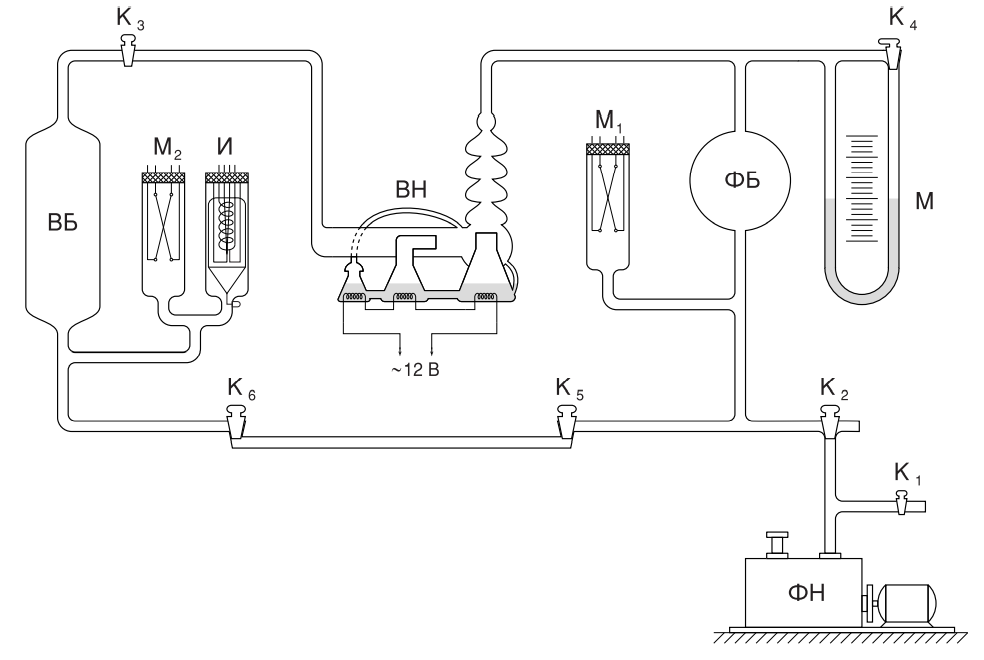
\includegraphics[width = 0.8\textwidth]{setup.PNG}
    \caption{Схема экспериментальной установки}
    \label{fig:setup}
\end{figure}

Использованная в работе экспериментальная установка изображена на рис. \ref{fig:setup}. Основным элементом
установки является трубка 1 с пористой перегородкой 2, через которую пропускается исследуемый газ. Трубка имеет длину 80 мм и сделана из нержавеющей стали, обладающей, как известно, малой теплопроводностью. Диаметр трубки $d = 3$ мм,
толщина стенок 0,2 мм. Пористая перегородка расположена в конце трубки и представляет собой стеклянную пористую пробку со множеством узких и длинных каналов. Пористость и толщина пробки ($l = 5$ мм) подобраны так, чтобы обеспечить оптимальный поток газа при перепаде давлений $ \Delta P = 4$ атм (расход газа составляет около 10 см$^3$/с); при этом в результате эффекта Джоуля–Томсона создается достаточная разность температур.

Углекислый газ под повышенным давлением поступает в трубку через змеевик 5 из балластного баллона 6. Медный змеевик омывается водой и нагревает медленно протекающий через него газ до температуры воды в термостате. Температура воды измеряется термометром T$_\text{в}$, помещенным в термостате. Требуемая температура воды устанавливается и поддерживается во время эксперимента при помощи контактного термометра T$_\text{к}$. Давление газа в трубке измеряется манометром М и регулируется вентилем В (при открывании вентиля В, т. е. при повороте ручки против часовой стрелки, давление $P_1$ повышается). Манометр М измеряет разность между давлением внутри трубки и наружным (атмосферным) давлением. Так как углекислый газ после пористой перегородки выходит в область с атмосферным давлением $P_2$, то этот манометр непосредственно измеряет перепад давления на входе и на выходе трубки. 

Разность температур газа до перегородки и после нее измеряется дифференциальной термопарой медь — константан. Константановая проволока диаметром 0,1 мм соединяет спаи 8 и 9, а медные проволоки (того же диаметра) подсоединены к цифровому вольтметру 7. Отвод тепла через проволоку столь малого сечения пренебрежимо мал. График зависимости разности температур от разности показаний вольтметра изображена на рис. \ref{graph0} Для уменьшения теплоотвода трубка с пористой перегородкой помещена в трубу Дьюара 3, стенки которой посеребрены, для уменьшения теплоотдачи, связанной с излучением. Для уменьшения теплоотдачи за счет конвекции один конец трубы Дьюара уплотнен кольцом 4, а другой закрыт пробкой 10 из пенопласта. Такая пробка практически не создает перепада давлений между внутренней полостью трубы и атмосферой.

\begin{figure}
\centering
\resizebox {0.55\textwidth} {!} {
\begin{tikzpicture}
\begin{axis}[ xlabel = {$t$, $^\text{o}$C}, ylabel = {$\Delta U/\Delta t$, мкВ/$^\text{o}$C}, xmin = 0, xmax = 50, ymin = 38, ymax = 43, legend style={legend style={at={(axis cs:332, 17)},anchor=north east}}]
\addplot[color=blue] coordinates{
(5, 38.9)
(45, 42.5)};

\end{axis}
\end{tikzpicture}
}
\caption{Зависимость теплоты образования единицы поверхности воды от температуры}
\label{graph0}
\end{figure}

\section{Оборудование и инструментальные погрешности}

\textbf{В работе использовались:} трубка с пористой перегородкой; труба Дьюара; термостат; термометры; дифференциальная термопара; микровольтметр; балластный баллон; манометр.

\textbf{Инструментальные погрешности:}

\begin{itemize}
    \item \textbf{Термометр в термостате:} $\Delta_T = 0,1$ К;
    \item \textbf{Термопара:} $\Delta_U = 1,0$ мкВ;
    \item \textbf{Манометр:} $\Delta_P = 0,05$ атм.
\end{itemize}

\section{Результаты измерений и обработка экспериментальных данных}

\subsection{Измерение коэффициента Джоуля-Томсона}

Измерения проводились для четырёх значений температуры от 20 до 35 $^\text{o}$C. Для каждого значения температуры были измерены показания термопары при отсутствии перепада давлений, а затем - для пяти различных значений перепадов давления. С помощью графика на рис. \ref{graph0} значения разности напряжений были преобразованы в значения разности температур. Полученные значения представлены в таблице \ref{tab:JTomson}

\begin{table}[]
    \centering
    \begin{tabular}{|c|c|c|c|c|c|}\hline
        $T$, К & $\Delta P$, атм & $U$, мкВ & $\Delta U$, мкВ & $\Delta T$, К & $\Delta T / \Delta P$, К/атм \\ \hline
        293,0 & 4,0 & -149,0 & -171,0 & -4,248 & -1,062 \\ \hline
        $\Delta U/\Delta T$, мкВ/$^\text{o}$C & 3,5 & -125,0 & -147,0 & -3,652 & -1,043 \\ \hline
        40,3 & 3,0 & -98,0 & -120,0 & -2,981 & -0,994 \\ \hline
        $U_0$, мкВ & 2,5 & -78,0 & -100,0 & -2,484 & -0,994 \\ \hline
        22,0 & 2,0 & -56,0 & -78,0 & -1,938 & -0,969 \\ \hline
        \multicolumn{6}{|c|}{} \\ \hline
        $T$, К & $\Delta P$, атм & $U$, мкВ & $\Delta U$, мкВ & $\Delta T$, К & $\Delta T / \Delta P$, К/атм \\ \hline
        298,0 & 4,0 & -136,0 & -153,0 & -3,759 & -0,940 \\ \hline
        $\Delta U/\Delta T$, мкВ/$^\text{o}$C & 3,5 & -115,0 & -132,0 & -3,243 & -0,927 \\ \hline
        40,7 & 3,0 & -92,0 & -109,0 & -2,678 & -0,893 \\ \hline
        $U_0$, мкВ & 2,5 & -73,0 & -90,0 & -2,211 & -0,885 \\ \hline
        17,0 & 2,0 & -56,0 & -73,0 & -1,794 & -0,897 \\ \hline
        \multicolumn{6}{|c|}{} \\ \hline
        $T$, К & $\Delta P$, атм & $U$, мкВ & $\Delta U$, мкВ & $\Delta T$, К & $\Delta T / \Delta P$, К/атм \\ \hline
        303,0 & 4,0 & -130,0 & -151,0 & -3,670 & -0,917 \\ \hline
        $\Delta U/\Delta T$, мкВ/$^\text{o}$C & 3,5 & -108,0 & -129,0 & -3,135 & -0,896 \\ \hline
        41,2 & 3,0 & -86,0 & -107,0 & -2,600 & -0,867 \\ \hline
        $U_0$, мкВ & 2,5 & -67,0 & -88,0 & -2,139 & -0,855 \\ \hline
        21,0 & 2,0 & -50,0 & -71,0 & -1,725 & -0,863 \\ \hline
        \multicolumn{6}{|c|}{} \\ \hline
        $T$, К & $\Delta P$, атм & $U$, мкВ & $\Delta U$, мкВ & $\Delta T$, К & $\Delta T / \Delta P$, К/атм \\ \hline
        308,0 & 4,0 & -127,0 & -147,0 & -3,534 & -0,883 \\ \hline
        $\Delta U/\Delta T$, мкВ/$^\text{o}$C & 3,5 & -105,0 & -125,0 & -3,005 & -0,859 \\ \hline
        41,6 & 3,0 & -80,0 & -100,0 & -2,404 & -0,801 \\ \hline
        $U_0$, мкВ & 2,5 & -65,0 & -85,0 & -2,043 & -0,817 \\ \hline
        20,0 & 2,0 & -42,0 & -62,0 & -1,490 & -0,745 \\ \hline
        \end{tabular}
    \caption{Результаты измерения величины эффекта Джоуля-Томсона}
    \label{tab:JTomson}
\end{table}

Систематические погрешности вычисленных величин равны

\begin{equation}
    \sigma^\text{сист}_{\Delta T} = \frac{\Delta_U}{\Delta U / \Delta T} \approx 0,025 \text{ К}; 
\end{equation}

\begin{equation}
    \sigma^\text{сист}_{\Delta T/\Delta P} = \frac{\Delta T}{\Delta P} \sqrt{(\frac{\Delta_P}{\Delta P})^2 + (\frac{\sigma^\text{сист}_{\Delta T}}{\Delta T})^2} \approx 0,023 \text{ К/атм.}
\end{equation}

Далее для каждого значения температуры вычислено среднее значение коэффициента Джоуля-Томсона $\overline{(\frac{\Delta T}{\Delta P})}$. Случайная и полная погрешности определения данного коэффициента вычисляются по формулам

\begin{equation}
        \sigma^\text{случ}_{\Delta T/\Delta P} = \sqrt{\frac{1}{N(N-1)} \sum\limits_{i = 1}^N((\frac{\Delta T}{\Delta P})_i - \overline{(\frac{\Delta T}{\Delta P})})^2};
\end{equation}

\begin{equation}
    \sigma^\text{полн}_{\Delta T/\Delta P} = \sqrt{(\sigma^\text{случ}_{\Delta T/\Delta P})^2 + (\sigma^\text{сист}_{\Delta T/\Delta P})^2}.
\end{equation}

Результаты вычисления средних значений коэффициентов Джоуля-Томсона и их погрешностей представлены в таблице \ref{tab:medKoeffs}.

\begin{table}[]
    \centering
    \begin{tabular}{|c|c|c|c|c|c|}\hline
        $T$, К & $\overline{(\Delta T/\Delta P)}$, К/атм & $\sigma^\text{случ}_{\Delta T/\Delta P}$, К/атм & $\sigma^\text{полн}_{\Delta T/\Delta P}$, К/атм \\ \hline
        293 & -1,012 & 0,017 & 0,029 \\ \hline
        298 & -0,908 & 0,011 & 0,025 \\ \hline
        303 & -0,880 & 0,012 & 0,026 \\ \hline
        308 & -0,821 & 0,024 & 0,033 \\ \hline
        \end{tabular}
    \caption{Коэффициенты Джоуля-Томсона при разных температурах и их погрешности}
    \label{tab:medKoeffs}
\end{table}

\subsection{Вычисление параметров газа Ван-дер-Ваальса}

Чтобы определить коэффициенты $a$ и $b$ в уравнении состояния газа Ван-дер-Ваальса, объединим выражения \eqref{mainEq} для двух температур газа в систему:

\begin{equation*}
 \begin{cases}
   (\Delta T/\Delta P)_1 = \frac{(2a/RT_1) - b}{C_P}; \\
   (\Delta T/\Delta P)_2 = \frac{(2a/RT_2) - b}{C_P}.
 \end{cases}
\end{equation*}

Отсюда получим выражения для коэффициентов:

\begin{equation*}
 \begin{cases}
   a = \frac{C_P R}{2} \cdot \frac{(\Delta T/\Delta P)_1 - (\Delta T/\Delta P)_2}{T_1^{-1} - T_2^{-1}}; \\
   b = \frac{2a}{RT_1} - C_P (\Delta T/\Delta P)_1.
 \end{cases}
\end{equation*}

Систематическая погрешность вычисления $a$ и $b$ определена как

\begin{equation}
    \sigma_a^\text{сист} = a\sqrt{2(\frac{\sigma_{\Delta T/\Delta P}}{(\Delta T/\Delta P)})^2 + 2(\frac{\Delta_T}{T})^2};
\end{equation}

\begin{equation}
    \sigma_b^\text{сист} = b \sqrt{(\frac{\sigma_a}{a})^2 + (\frac{\Delta_T}{T})^2 + (\frac{\sigma_{\Delta T/\Delta P}}{\Delta T/\Delta P})^2}.
\end{equation}

Данные коэффициенты были вычислены для трёх пар температур. По найденным коэффициентам вычислены соответствующие значения критической температуры углекислого газа. Систематическая погрешность вычисления критической температуры определена как

\begin{equation}
    \sigma_T = T_\text{кр} \sqrt{(\frac{\sigma_a}{a})^2 + (\frac{\sigma_b}{b})^2}.
\end{equation}

Результаты вычислений представлены в таблице .

\begin{table}[]
    \centering
    \begin{tabular}{|c|c|c|c|c|c|c|c|}\hline
        $T_1$, К & $T_2$, К & $a$, Па$\cdot$м$^6$/моль$^2$ & $b$, $10^{-3}$ м$^3$/моль & $\sigma_a$, Па$\cdot$м$^6$/моль$^2$ & $\sigma_b$, $10^{-3}$ м$^3$/моль & $T_\text{кр}$, К & $\sigma_T$, К \\ \hline
        293 & 298 & 2,99 & 2,05 & 0,12 & 0,11 & 52 & 3 \\ \hline
        298 & 303 & 0,84 & 0,32 & 0,03 & 0,02 & 93 & 6 \\ \hline
        303 & 308 & 1,79 & 1,07 & 0,08 & 0,06 & 59 & 4 \\ \hline
        \end{tabular}
    \caption{Коэффициенты газа Ван-дер-Ваальса и значения критической температуры}
    \label{tab:badResults}
\end{table}

\section{Обсуждение результатов и выводы}

В работе получены следующие значения критической температуры углекислого газа:

\begin{itemize}
    \item $T_\text{кр} = 52 \pm 3$ К;
    \item $T_\text{кр} = 93 \pm 6$ К;
    \item $T_\text{кр} = 59 \pm 4$ К.
\end{itemize}

Табличное значение критической температуры углекислого газа равно $T_\text{кр} \approx 304$ К, что почти на порядок больше полученных значений. Из этого можно сделать вывод о том, что данная методика изучения реального газа не применима. Действительно, модель газа Ван-дер-Ваальса позволяет лишь качественно объяснить свойства реальных газов, однако она очень неточно описывает их количественно. Коэффициенты в уравнении состояния \eqref{vdv} полагаются постоянными, в то время как опыт показал, что их значения зависят от состояния газа. Также необходимо учитывать, что измерения проводились вблизи критической температуры углекислого газа, поэтому могли возникнуть дополнительные неточности при применении уравнения Ван-дер-Ваальса.

Также по результатам работы видно, что данная методика измерений не применима совместно с дифференциальной моделью эффекта Джоуля-Томсона, т.к. данная модель рассматривает малые приращения температуры и давления, которые невозможно с достаточной точностью измерить имеющимися в лаборатории приборами. Из-за этого коэффициент Джоуля-Томсона невозможно верно оценить с помощью аппроксимации.

Опыт показал, однако, что качественное описание газа моделью Ван-дер-Ваальса верно: реальный газ при дросселировании действительно охлаждается, причём вблизи комнатной температуры величина эффекта действительно практически не зависит от перепада давления. Данный опыт продемонстрировал отличие реального газа от идеального. 

\end{document}